\label{appendix:presion}

Este apéndice está destinado a mostrar una definición alternativa de la ``presión local". Se mostrará un ejemplo teórico (partículas en hilera) para aclarar algunos conceptos y por último se presentarán muestras de ``performance" con el fin de evidenciar la similitud con la definición de presión de Helbing y el rendimiento que tiene el cálculo de la presión según esta definición alternativa.  
\\

\section{Presión local}

A pesar de que la fuerza de deseo es una fuerza unilateral (\textit{i.e.} partícula auto-impulsada), la ecuación de movimiento continúa siendo válida, y por lo tanto, podemos derivar la relación del virial~\cite{lion}, para un conjunto de $N$ peatones dentro del área $\mathcal{A}$.

\begin{equation}
 \bigg\langle\displaystyle\sum_{i=1}^N\displaystyle\frac{p_i^2}{m_i} + 
\displaystyle\sum_{i=1}^N 
\mathbf{r}_i\cdot\mathbf{f}_i\bigg\rangle=-2\mathcal{PA}\label{virial1}
\end{equation}


$p_i$  y $\mathbf{f}_i$ son el momento y la fuerza total actuando sobre el individuo $i$. La fuerza $\mathbf{f}_i$ no contempla la interacción con las paredes.  $\langle\cdot\rangle$ corresponde al valor medio en el tiempo. El lado derecho de la ecuación $-2\mathcal{PA}$ es la presión global en el perímetro del recinto $\mathcal{A}$. Este término es negativo porque el producto de $\mathbf{r}_{iW}\cdot\mathbf{f}_s^{(iW)}$ es positivo y pasa al lado derecho con signo negativo (siendo $2\mathcal{PA}>0$). En la bibliografía, el término $2\mathcal{PA}$ aparece con signo positivo ya que se considera la presión que se ejerce sobre la pared y no la presión que se ejerce sobre las partículas, en contacto con ella, como en este caso.  \\
La presión local para un peatón ($i$) está asociada a las fuerzas (por unidad de área) actuando sobre él y debidas a los individuos que lo rodean. Según la Ref.~\cite{lion} se puede definir una ``función de presión social" $P_i$ como:\\

\begin{equation}
2P_iA_i=\displaystyle\frac{p_i^2}{m_i} + \frac{1}{2}
\displaystyle\sum_{j=1}^{N-1}
\mathbf{r}_{ij}\cdot\mathbf{f}_s^{(ij)}\label{pa}
\end{equation}

donde $A_i$ es el área que encierra al peatón $i$ y 
$\mathbf{r}_{ij}=\mathbf{r}_{i}-\mathbf{r}_j$ (la distancia
entre dos peatones en la dirección desde $j$ hacia $i$). Cabe destacar que el producto interno $\mathbf{r}_{ij}\cdot\mathbf{f}_s^{(ij)}$ siempre es positivo debido a la repulsión y es igual al producto escalar (positivo) $d_{ij}f_s^{(ij)}$. El factor 1/2 evita el doble conteo de las interacciones cuando se hace la suma de todos los $2P_iA_i$. Esta función de presión local contempla un término cinético que la definición de presión Helbing ignora. \\ 

El segundo término en la ecuación (\ref{virial1}) puede dividirse en la suma de productos internos $\mathbf{r}_i\cdot\mathbf{f}_d$ (deseo), 
$\mathbf{r}_i\cdot\mathbf{f}_s$ (social) y $\mathbf{r}_i\cdot\mathbf{f}_g$ (granular). De hecho, la suma del producto social depende de la distancia entre partículas $d_{ij}f_s^{(ij)}$, mientras que la parte granular no tiene ningún rol por su ortogonalidad ($\mathbf{r}_{ij}\cdot\mathbf{f}_g^{(ij)}=0$). Por lo tanto, la relación del virial (\ref{virial1}) se expresa \\  

\begin{equation}
 \displaystyle\sum_{i=1}^N\langle2P_iA_i 
\rangle=-2\mathcal{PA} -\displaystyle\sum_{i=1}^N \langle
\mathbf{r}_i\cdot\mathbf{f}_d^{(i)}\rangle\label{virial2}
\end{equation}

Hay que destacar que la ecuación (\ref{virial2}) se cumple ya sea si los peatones están en contacto o no. Esto significa que no se trata de una presión de contacto (habitual en los sistemas físicos tradicionales) sino de una presión que provoca una cambio en el patrón de movimiento del individuo.\\

La suma de fuerzas por unidad de circunferencia (\textit{i.e.} medida de presión según la Ref.~\cite{Helbing1}) es similar a la definición dada en (\ref{pa}) y que, a su vez, se sigue de la Ref.\cite{lion}. Comprobamos durante la investigación que ambas son proporcionales. En la sección \ref{Muestras de performace} se verifica la relación \eqref{virial2} a través de ejemplos particulares simulados.\\   

\section{\label{social_pressure} Individuos en hilera}

La figura ~\ref{hilera2} representa una hilera de individuos empujando hacia la derecha. La pared impide el movimiento de los peatones. Todos los individuos de la hilera están en su posición de equilibrio $x_1,x_2,...,x_{i},...x_N$, mientras que la pared está en la posición $x_0=0$. 

\begin{figure}[!htbp]
\center
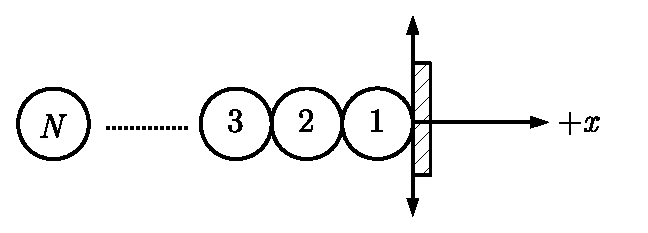
\includegraphics[scale=1]{figuras/hilera.eps}
\caption{\label{hilera2} Hilera de individuos empujando hacia la derecha. El eje horizontal indica la posición positiva. }
% done with figuras_presion.odg
\end{figure}

Los peatones empujan hacia la derecha gracias a la fuerza de deseo
$f_d^{(i)}=mv_d/\tau$, según la Ec.~(\ref{fdeseo}). La repulsión social balancea la fuerza de deseo, pero sólo se tiene en cuenta la interacción de los individuos en contacto (se desprecia la interacción de segundos vecinos). La Ec. ~\ref{eqn_6} muestra la ecuación de balance de cada individuo en la hilera. \\

\begin{equation}
 f_s^{(i,i+1)}-f_s^{(i,i-1)}+\displaystyle\frac{mv_d}{\tau}=0\label{eqn_6}
\end{equation}

siendo $f_s^{(i,j)}$ la fuerza repulsiva que siente el individuo $i$ debido a la presencia del peatón $j$. Cabe destacar que la condición de contorno para la posición $x_0=0$ es condición de Dirichlet, mientras que la condición en el otro extremo es una condición de Neumann $f_s^{(N,N+1)}=0$. Las fuerzas sobre los peatones se obtienen de forma recursiva a partir de la expresión~\ref{eqn_6}, empezando desde el extremo libre ($i=N$). El resultado es

\begin{equation}
f_s^{(i,i-1)}=(N-i+1)\,\displaystyle\frac{mv_d}{\tau}\ \ \ , \ \ \ 
i=1,....,N\label{eqn_7}
\end{equation}

con las correspondientes posiciones  $x_1,x_2,...,x_{i},...x_N$ obtenidas a partir de la sustitución de la fuerza social expresada en Ec.~\ref{fsocial}, comenzando en la posición de la pared.

\begin{equation} 
x_i=x_{i-1}-(r_{i}+r_{i-1})+B\,\ln\bigg[(N-i+1)\,\displaystyle\frac{mv_d}{A\tau}
\bigg]\label{eqn_8}
\end{equation}

La intuición sugiere que la presión que siente un peatón $P_i$ 
corresponde a las fuerzas actuando en él (por unidad de área) debido a los primeros vecinos. De la definición de "función de presión social" (\ref{pa}) se puede derivar

\begin{equation}
P_i=\displaystyle\frac{1}{2}\,\bigg[\displaystyle\frac{x_{i}-x_{i+1}}{2A_i}\,
f_s^ { (i , i+1) } +\displaystyle\frac { x_ {i-1}-x_{i}}{2A_i}\,f_s^{(i,i-1) 
}\bigg]\label{eqn_9}
\end{equation}

\vspace{3mm}

donde la magnitud $x_{ij}/2A_i$ corresponde a la inversa de la superficie efectiva del peatón. Para individuos modelados como círculos rígidos, la distancia entre peatones es $x_{ij}=2r_i$ y el área $A_i=\pi r_i^2$. Por lo tanto, 

\begin{equation}
P_i=\displaystyle\frac{1}{4\pi 
r_i}\,\bigg[f_s^ { (i , i+1) } +f_s^{(i,i-1)}\bigg]\label{eqn_10}
\end{equation}

como es de esperar para la presión del individuo. Notar que esta expresión, al igual que la definición de presión de Helbing tiene unidades de fuerza por unidad de longitud. \\


\section{\label{Muestras de performace} Muestras de performance} 

En esta sección se describirá el módulo creado para cuantificar la ``presión social" según esta definición alternativa. Luego se compararán las dos definiciones de presión a través de un ejemplo particular. Por último se mostrarán dos ejemplos para comprobar que la definición alternativa satisface la ecuación del virial. 

{\Large {\tt compute\_social\_pressure}}

Calcula la función de presión social de la expresión (\ref{pa}) despreciando el término cinético y el factor 1/2. Para cada timestep devuelve un vector con la presión que soporta cada peatón como consecuencia de la interacción con sus vecinos. Sólo se tienen en cuenta las presiones producidas por la repulsión de fuerza social, es decir, se ignoran las interacciones con las paredes así como el rozamiento entre individuos. Se desprecia el término cinético porque sólo cuando los individuos están amontonados (situación cuasi estática) el valor de presión es apreciable. En esta situación el término asociado a la repulsión social es al menos un orden de magnitud mayor que el término asociado a la energía cinética. \\

Con este módulo de presión se hicieron cálculos para comparar la ``definición alternativa" con la definición de presión de Helbing. En la figura \ref{comparacion} se muestra la presión en función de la distancia a la puerta para un recinto con 225 individuos a $v_d=4$~m/s. Los triángulos representan la presión según la Ec.~(\ref{phelbing}), mientras que los círculos la presión según Ec.~(\ref{pa}). Puede verse que ambas definiciones generan resultados similares. 

\begin{figure}[H]
    \centering
    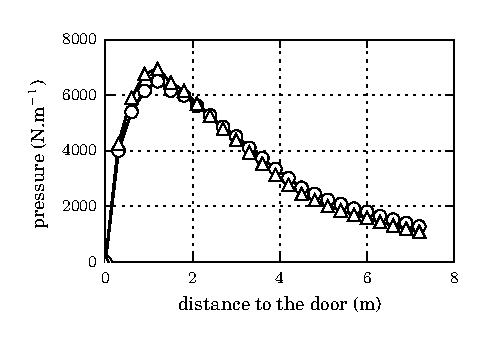
\includegraphics[scale=1]{figuras/fig16.eps}
    \caption[width=5cm]{Presión media en función de la distancia a la salida. El recinto era de $20\,\mathrm{m}\times20\,\mathrm{m}$, con una puerta de 1,2~m de ancho. Se realizaron promedios sobre 30 procesos de evacuación, hasta que evacuaron 100 individuos. La velocidad de deseo era $v_d=4\,$m/s. La distancia a la puerta fue segmentada en intervalos de $0,3$~m.  El $\bigcirc$  corresponde al valor medio de la presión según Ec. \ref{pa}, despreciando la parte cinética ($p_i=0$) y $\mathcal{A}_i=\pi r_i^2$. El símbolo $\bigtriangleup$ corresponde a la presión computada según la Ec. \ref{phelbing}. }
    \label{comparacion}
\end{figure}

A continuación se mostrarán los ejemplos que demuestran cómo el módulo    {\tt compute\_social\_pressure} genera resultados que convalidan con las ecuaciones teóricas.  

\subsection{Partículas centradas}

Se simuló un conjunto de 19 partículas cuyo ``target" es el origen de coordenadas (partícula central en la figura \ref{central}). Con una velocidad de deseo $v_d=4$~m/s en módulo. En el estado estacionario la disposición de las partículas es tal como se muestra en la figura \ref{central} . Las partículas se encuentran casi estáticas (sus fuerzas de deseo se compensan con la repulsión social); pero aun así, poseen una pequeña oscilación en torno a la posición de equilibrio. 

\begin{figure}[H]
    \centering
        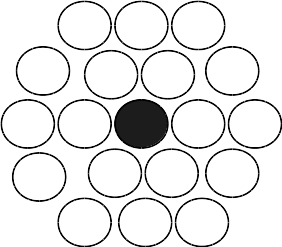
\includegraphics[scale=0.5]{figuras/central.png}
    \caption[width=5cm]{Esquema de las partículas. Partícula central (coloreada de negro) rodeada por 6 primeros vecinos y doce segundos vecinos.}
    \label{central}
\end{figure}


El resultado de esta simulación es el conjunto de valores que se exhiben en las tablas de abajo. Éstos son la distancia al origen y la presión social que siente cada individuo. 

%\begin{table}[H]
\begin{center}
%\caption{Resultados numéricos de la simulación.}
\label{my-label}
\begin{tabular}{|l|l|}
\hline
Distancia (m) & Presión (N/m) \\ \hline
1,48          & 664,0       \\ \hline
1,26          & 999,9       \\ \hline
1,49          & 653,3       \\ \hline
1,48          & 664,0       \\ \hline
1,27          & 988,7       \\ \hline
0,7           & 1820,5       \\ \hline
0,7           & 1820,9       \\ \hline
0,0           & 2340,2       \\ \hline
0,7           & 1829,9       \\ \hline
0,7           & 1833,5       \\ \hline
\end{tabular}
\quad
\begin{tabular}{|l|l|}
\hline
Distancia (m) & Presión (N/m) \\ \hline
1,26          & 989,8       \\ \hline
1,49          & 655,2       \\ \hline
1,26          & 991,9       \\ \hline
1,49          & 653,7        \\ \hline
0,7           & 1828,0       \\ \hline
1,26          & 1004,1       \\ \hline
0,7           & 1833,6       \\ \hline
1,48          & 663,1       \\ \hline
1,26          & 1002,1       \\ \hline
\end{tabular}
%\end{table}
\end{center}


Sumar todos los valores de presión social y dividir por dos da como resultado el lado izquierdo de la ecuación (\ref{virial2}).
\begin{equation}
 \displaystyle\sum_{i=1}^N\langle2P_iA_i\rangle = 11618.6\ \text{N/m}
\end{equation}

La suma de todas las distancias multiplicada por la fuerza de deseo $f_d=mv_d/\tau$ da como resultado el lado derecho (despreciando el primer término porque no hay interacción con paredes):

\begin{equation}
 -2\mathcal{PA} -\displaystyle\sum_{i=1}^N \langle
\mathbf{r}_i\cdot\mathbf{f}_d^{(i)}\rangle\ =  11580.8\ \text{N/m}
\end{equation}

Ambos valores son cercanos. Por lo tanto, el resultado de esta simulación verifica la relación del virial (\ref{virial2}).


\subsection{Partículas en hilera}

Se creó un código que mide la presión que soportan los individuos dispuestos en hilera como muestra la figura \ref{hilera}.  

\begin{figure}[!htbp]
\center
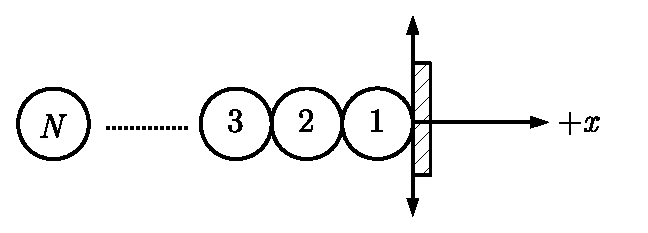
\includegraphics[scale=1]{figuras/hilera.eps}
\caption[width=5cm]{Hilera de individuos empujando a la derecha. Situación estática donde las fuerzas de deseo de cada individuo se compensan con la repulsión social.}
\label{hilera}
% done with figuras_presion.odg
\end{figure}

Los resultados se muestran en la tabla \ref{simulados}. La misma está ordenada del individuo más cercano al más lejano de la pared. La presión disminuye conforme se alejan de la pared y el valor de presión aumenta con la cantidad de individuos.\\
En la tabla \ref{teoricos} se muestran valores de presión teóricos (calculados a partir de las fórmulas \ref{eqn_7}, \ref{eqn_8} y \ref{eqn_9}). Las magnitudes de presión son comparables a las simuladas y el comportamiento a grandes rasgos es similar (las partículas más presionadas son las que se encuentran más cerca de la pared y aumentar N aumenta la presión general)  

\begin{table}[h!]
\caption {Valores simulados de $4P_iA_i$ para $v_d=4\,$m/s.}
\label{simulados}
\begin{center}
\begin{tabular}{|l|cccccc|}
\hline
      & \multicolumn{6}{c|}{$N$} \\
\hline
$i$   &  1   &   2    &  3       &  4     &  5     &   6     \\
\hline
 1    &  --- &  ---   &  ---     & ---    & ---    & ---     \\
 2    &      &  393.2 &  1116.7  & 1751.4 & 2362.2 & 2927.0  \\
 3    &      &        &  393.03  & 1113.8 & 1761.7 & 2355.1  \\
 4    &      &        &          & 391.45 & 1120.3 & 1755.4  \\
 5    &      &        &          &        & 394.03 & 1117.0  \\
 6    &      &        &          &        &        & 393.03  \\
\hline
\end{tabular}
\end{center}
\end{table}



\begin{table}[h!]
\caption {Valores teóricos de $4P_iA_i$ para $v_d=4\,$m/s.}
\label{teoricos}
\begin{center}
\begin{tabular}{|l|cccccc|}
\hline
      & \multicolumn{6}{c|}{$N$} \\
\hline
$i$   &  1         &   2        &  3       &  4     &  5     &   6   \\
\hline
 1    &  225.03    &  780.98    &  1251.4  & 1683.1 & 2088.3 & 2473.2 \\
 2    &            &  393.03    &  1117.0  & 1755.4 & 2355.1 & 2928.3 \\
 3    &            &            &  393.03  & 1117.0 & 1755.4 & 2355.1 \\
 4    &            &            &          & 393.03 & 1117.0 & 1755.4 \\
 5    &            &            &          &        & 393.03 & 1117.0 \\
 6    &            &            &          &        &        & 393.03 \\
\hline
\end{tabular}
\end{center}
\end{table}


En esta sección se verificó que los resultados simulados satisfacen la relación del virial (partículas centradas) y a su vez concuerdan con los cálculos teóricos (partículas en hilera)


